\documentclass[1p]{elsarticle_modified}
%\bibliographystyle{elsarticle-num}

%\usepackage[colorlinks]{hyperref}
%\usepackage{abbrmath_seonhwa} %\Abb, \Ascr, \Acal ,\Abf, \Afrak
\usepackage{amsfonts}
\usepackage{amssymb}
\usepackage{amsmath}
\usepackage{amsthm}
\usepackage{scalefnt}
\usepackage{amsbsy}
\usepackage{kotex}
\usepackage{caption}
\usepackage{subfig}
\usepackage{color}
\usepackage{graphicx}
\usepackage{xcolor} %% white, black, red, green, blue, cyan, magenta, yellow
\usepackage{float}
\usepackage{setspace}
\usepackage{hyperref}

\usepackage{tikz}
\usetikzlibrary{arrows}

\usepackage{multirow}
\usepackage{array} % fixed length table
\usepackage{hhline}

%%%%%%%%%%%%%%%%%%%%%
\makeatletter
\renewcommand*\env@matrix[1][\arraystretch]{%
	\edef\arraystretch{#1}%
	\hskip -\arraycolsep
	\let\@ifnextchar\new@ifnextchar
	\array{*\c@MaxMatrixCols c}}
\makeatother %https://tex.stackexchange.com/questions/14071/how-can-i-increase-the-line-spacing-in-a-matrix
%%%%%%%%%%%%%%%

\usepackage[normalem]{ulem}

\newcommand{\msout}[1]{\ifmmode\text{\sout{\ensuremath{#1}}}\else\sout{#1}\fi}
%SOURCE: \msout is \stkout macro in https://tex.stackexchange.com/questions/20609/strikeout-in-math-mode

\newcommand{\cancel}[1]{
	\ifmmode
	{\color{red}\msout{#1}}
	\else
	{\color{red}\sout{#1}}
	\fi
}

\newcommand{\add}[1]{
	{\color{blue}\uwave{#1}}
}

\newcommand{\replace}[2]{
	\ifmmode
	{\color{red}\msout{#1}}{\color{blue}\uwave{#2}}
	\else
	{\color{red}\sout{#1}}{\color{blue}\uwave{#2}}
	\fi
}

\newcommand{\Sol}{\mathcal{S}} %segment
\newcommand{\D}{D} %diagram
\newcommand{\A}{\mathcal{A}} %arc


%%%%%%%%%%%%%%%%%%%%%%%%%%%%%5 test

\def\sl{\operatorname{\textup{SL}}(2,\Cbb)}
\def\psl{\operatorname{\textup{PSL}}(2,\Cbb)}
\def\quan{\mkern 1mu \triangleright \mkern 1mu}

\theoremstyle{definition}
\newtheorem{thm}{Theorem}[section]
\newtheorem{prop}[thm]{Proposition}
\newtheorem{lem}[thm]{Lemma}
\newtheorem{ques}[thm]{Question}
\newtheorem{cor}[thm]{Corollary}
\newtheorem{defn}[thm]{Definition}
\newtheorem{exam}[thm]{Example}
\newtheorem{rmk}[thm]{Remark}
\newtheorem{alg}[thm]{Algorithm}

\newcommand{\I}{\sqrt{-1}}
\begin{document}

%\begin{frontmatter}
%
%\title{Boundary parabolic representations of knots up to 8 crossings}
%
%%% Group authors per affiliation:
%\author{Yunhi Cho} 
%\address{Department of Mathematics, University of Seoul, Seoul, Korea}
%\ead{yhcho@uos.ac.kr}
%
%
%\author{Seonhwa Kim} %\fnref{s_kim}}
%\address{Center for Geometry and Physics, Institute for Basic Science, Pohang, 37673, Korea}
%\ead{ryeona17@ibs.re.kr}
%
%\author{Hyuk Kim}
%\address{Department of Mathematical Sciences, Seoul National University, Seoul 08826, Korea}
%\ead{hyukkim@snu.ac.kr}
%
%\author{Seokbeom Yoon}
%\address{Department of Mathematical Sciences, Seoul National University, Seoul, 08826,  Korea}
%\ead{sbyoon15@snu.ac.kr}
%
%\begin{abstract}
%We find all boundary parabolic representation of knots up to 8 crossings.
%
%\end{abstract}
%\begin{keyword}
%    \MSC[2010] 57M25 
%\end{keyword}
%
%\end{frontmatter}

%\linenumbers
%\tableofcontents
%
\newcommand\colored[1]{\textcolor{white}{\rule[-0.35ex]{0.8em}{1.4ex}}\kern-0.8em\color{red} #1}%
%\newcommand\colored[1]{\textcolor{white}{ #1}\kern-2.17ex	\textcolor{white}{ #1}\kern-1.81ex	\textcolor{white}{ #1}\kern-2.15ex\color{red}#1	}

{\Large $\underline{12a_{0880}~(K12a_{0880})}$}

\setlength{\tabcolsep}{10pt}
\renewcommand{\arraystretch}{1.6}
\vspace{1cm}\begin{tabular}{m{100pt}>{\centering\arraybackslash}m{274pt}}
\multirow{5}{120pt}{
	\centering
	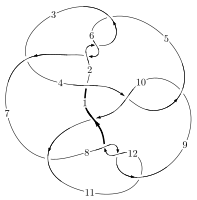
\includegraphics[width=112pt]{../../../GIT/diagram.site/Diagrams/png/1681_12a_0880.png}\\
\ \ \ A knot diagram\footnotemark}&
\allowdisplaybreaks
\textbf{Linearized knot diagam} \\
\cline{2-2}
 &
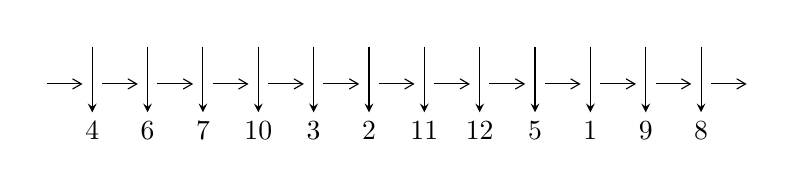
\begin{tikzpicture}[x=20pt, y=17pt]
	% nodes
	\node (C0) at (0, 0) {};
	\node (C1) at (1, 0) {};
	\node (C1U) at (1, +1) {};
	\node (C1D) at (1, -1) {4};

	\node (C2) at (2, 0) {};
	\node (C2U) at (2, +1) {};
	\node (C2D) at (2, -1) {6};

	\node (C3) at (3, 0) {};
	\node (C3U) at (3, +1) {};
	\node (C3D) at (3, -1) {7};

	\node (C4) at (4, 0) {};
	\node (C4U) at (4, +1) {};
	\node (C4D) at (4, -1) {10};

	\node (C5) at (5, 0) {};
	\node (C5U) at (5, +1) {};
	\node (C5D) at (5, -1) {3};

	\node (C6) at (6, 0) {};
	\node (C6U) at (6, +1) {};
	\node (C6D) at (6, -1) {2};

	\node (C7) at (7, 0) {};
	\node (C7U) at (7, +1) {};
	\node (C7D) at (7, -1) {11};

	\node (C8) at (8, 0) {};
	\node (C8U) at (8, +1) {};
	\node (C8D) at (8, -1) {12};

	\node (C9) at (9, 0) {};
	\node (C9U) at (9, +1) {};
	\node (C9D) at (9, -1) {5};

	\node (C10) at (10, 0) {};
	\node (C10U) at (10, +1) {};
	\node (C10D) at (10, -1) {1};

	\node (C11) at (11, 0) {};
	\node (C11U) at (11, +1) {};
	\node (C11D) at (11, -1) {9};

	\node (C12) at (12, 0) {};
	\node (C12U) at (12, +1) {};
	\node (C12D) at (12, -1) {8};
	\node (C13) at (13, 0) {};

	% arrows
	\draw[->,>={angle 60}]
	(C0) edge (C1) (C1) edge (C2) (C2) edge (C3) (C3) edge (C4) (C4) edge (C5) (C5) edge (C6) (C6) edge (C7) (C7) edge (C8) (C8) edge (C9) (C9) edge (C10) (C10) edge (C11) (C11) edge (C12) (C12) edge (C13) ;	\draw[->,>=stealth]
	(C1U) edge (C1D) (C2U) edge (C2D) (C3U) edge (C3D) (C4U) edge (C4D) (C5U) edge (C5D) (C6U) edge (C6D) (C7U) edge (C7D) (C8U) edge (C8D) (C9U) edge (C9D) (C10U) edge (C10D) (C11U) edge (C11D) (C12U) edge (C12D) ;
	\end{tikzpicture} \\
\hhline{~~} \\& 
\textbf{Solving Sequence} \\ \cline{2-2} 
 &
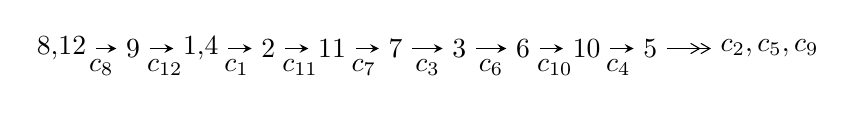
\begin{tikzpicture}[x=23pt, y=7pt]
	% node
	\node (A0) at (-1/8, 0) {8,12};
	\node (A1) at (1, 0) {9};
	\node (A2) at (33/16, 0) {1,4};
	\node (A3) at (25/8, 0) {2};
	\node (A4) at (33/8, 0) {11};
	\node (A5) at (41/8, 0) {7};
	\node (A6) at (49/8, 0) {3};
	\node (A7) at (57/8, 0) {6};
	\node (A8) at (65/8, 0) {10};
	\node (A9) at (73/8, 0) {5};
	\node (C1) at (1/2, -1) {$c_{8}$};
	\node (C2) at (3/2, -1) {$c_{12}$};
	\node (C3) at (21/8, -1) {$c_{1}$};
	\node (C4) at (29/8, -1) {$c_{11}$};
	\node (C5) at (37/8, -1) {$c_{7}$};
	\node (C6) at (45/8, -1) {$c_{3}$};
	\node (C7) at (53/8, -1) {$c_{6}$};
	\node (C8) at (61/8, -1) {$c_{10}$};
	\node (C9) at (69/8, -1) {$c_{4}$};
	\node (A10) at (11, 0) {$c_{2},c_{5},c_{9}$};

	% edge
	\draw[->,>=stealth]	
	(A0) edge (A1) (A1) edge (A2) (A2) edge (A3) (A3) edge (A4) (A4) edge (A5) (A5) edge (A6) (A6) edge (A7) (A7) edge (A8) (A8) edge (A9) ;
	\draw[->>,>={angle 60}]	
	(A9) edge (A10);
\end{tikzpicture} \\ 

\end{tabular} \\

\footnotetext{
The image of knot diagram is generated by the software ``\textbf{Draw programme}" developed by Andrew Bartholomew(\url{http://www.layer8.co.uk/maths/draw/index.htm\#Running-draw}), where we modified some parts for our purpose(\url{https://github.com/CATsTAILs/LinksPainter}).
}\phantom \\ \newline 
\centering \textbf{Ideals for irreducible components\footnotemark of $X_{\text{par}}$} 
 
\begin{align*}
I^u_{1}&=\langle 
u^{15}+u^{14}+7 u^{13}+6 u^{12}+17 u^{11}+12 u^{10}+14 u^9+6 u^8-3 u^7-6 u^6-5 u^5-3 u^4+2 u^3+2 u^2+b+u-1,\\
\phantom{I^u_{1}}&\phantom{= \langle  }- u^{15}- u^{14}-7 u^{13}-6 u^{12}-17 u^{11}-12 u^{10}-14 u^9-6 u^8+3 u^7+6 u^6+5 u^5+3 u^4- u^3-2 u^2+a+u+1,\\
\phantom{I^u_{1}}&\phantom{= \langle  }u^{17}+u^{16}+\cdots+2 u-1\rangle \\
I^u_{2}&=\langle 
6 u^{71}+3 u^{70}+\cdots+2 b+6,\;13 u^{71}+37 u^{70}+\cdots+2 a+22,\;u^{72}+3 u^{71}+\cdots+4 u+1\rangle \\
I^u_{3}&=\langle 
u^2+b,\;a+1,\;u^3- u^2+2 u-1\rangle \\
I^u_{4}&=\langle 
- u^2 a+b,\;- u^2 a+a^2+u^2-2 a+2,\;u^3- u^2+2 u-1\rangle \\
\\
\end{align*}
\raggedright * 4 irreducible components of $\dim_{\mathbb{C}}=0$, with total 98 representations.\\
\footnotetext{All coefficients of polynomials are rational numbers. But the coefficients are sometimes approximated in decimal forms when there is not enough margin.}
\newpage
\renewcommand{\arraystretch}{1}
\centering \section*{I. $I^u_{1}= \langle u^{15}+u^{14}+\cdots+b-1,\;- u^{15}- u^{14}+\cdots+a+1,\;u^{17}+u^{16}+\cdots+2 u-1 \rangle$}
\flushleft \textbf{(i) Arc colorings}\\
\begin{tabular}{m{7pt} m{180pt} m{7pt} m{180pt} }
\flushright $a_{8}=$&$\begin{pmatrix}1\\0\end{pmatrix}$ \\
\flushright $a_{12}=$&$\begin{pmatrix}0\\u\end{pmatrix}$ \\
\flushright $a_{9}=$&$\begin{pmatrix}1\\u^2\end{pmatrix}$ \\
\flushright $a_{1}=$&$\begin{pmatrix}- u\\u\end{pmatrix}$ \\
\flushright $a_{4}=$&$\begin{pmatrix}u^{15}+u^{14}+\cdots- u-1\\- u^{15}- u^{14}+\cdots- u+1\end{pmatrix}$ \\
\flushright $a_{2}=$&$\begin{pmatrix}- u^{15}- u^{14}+\cdots- u^2- u\\u^{15}+u^{14}+\cdots+u^2+u\end{pmatrix}$ \\
\flushright $a_{11}=$&$\begin{pmatrix}u\\u^3+u\end{pmatrix}$ \\
\flushright $a_{7}=$&$\begin{pmatrix}- u^4- u^2+1\\- u^6-2 u^4- u^2\end{pmatrix}$ \\
\flushright $a_{3}=$&$\begin{pmatrix}u^{15}+u^{14}+\cdots+2 u^2-1\\- u^{15}- u^{14}+\cdots- u+1\end{pmatrix}$ \\
\flushright $a_{6}=$&$\begin{pmatrix}u^{16}+u^{15}+\cdots+u^3+1\\- u^{16}- u^{15}+\cdots- u^3-2 u^2\end{pmatrix}$ \\
\flushright $a_{10}=$&$\begin{pmatrix}u^5+2 u^3+u\\- u^5- u^3+u\end{pmatrix}$ \\
\flushright $a_{5}=$&$\begin{pmatrix}- u^{12}- u^{11}-6 u^{10}-5 u^9-13 u^8-8 u^7-11 u^6-3 u^5-2 u^4+u^3- u-1\\u^{12}+u^{11}+5 u^{10}+5 u^9+8 u^8+8 u^7+3 u^6+3 u^5- u^4- u^3+u^2+u\end{pmatrix}$\\&\end{tabular}
\flushleft \textbf{(ii) Obstruction class $= -1$}\\~\\
\flushleft \textbf{(iii) Cusp Shapes $= -4 u^{16}-4 u^{15}-32 u^{14}-30 u^{13}-98 u^{12}-86 u^{11}-136 u^{10}-108 u^9-70 u^8-40 u^7+10 u^6+18 u^5+12 u^4-2 u^3-4 u^2-8 u-12$}\\~\\
\newpage\renewcommand{\arraystretch}{1}
\flushleft \textbf{(iv) u-Polynomials at the component}\newline \\
\begin{tabular}{m{50pt}|m{274pt}}
Crossings & \hspace{64pt}u-Polynomials at each crossing \\
\hline $$\begin{aligned}c_{1},c_{10}\end{aligned}$$&$\begin{aligned}
&u^{17}-3 u^{16}+\cdots-13 u^2+1
\end{aligned}$\\
\hline $$\begin{aligned}c_{2},c_{5},c_{6}\\c_{8},c_{11},c_{12}\end{aligned}$$&$\begin{aligned}
&u^{17}- u^{16}+\cdots+2 u+1
\end{aligned}$\\
\hline $$\begin{aligned}c_{3},c_{7}\end{aligned}$$&$\begin{aligned}
&u^{17}+u^{16}+\cdots-2 u+1
\end{aligned}$\\
\hline $$\begin{aligned}c_{4},c_{9}\end{aligned}$$&$\begin{aligned}
&u^{17}-7 u^{16}+\cdots-24 u+8
\end{aligned}$\\
\hline
\end{tabular}\\~\\
\newpage\renewcommand{\arraystretch}{1}
\flushleft \textbf{(v) Riley Polynomials at the component}\newline \\
\begin{tabular}{m{50pt}|m{274pt}}
Crossings & \hspace{64pt}Riley Polynomials at each crossing \\
\hline $$\begin{aligned}c_{1},c_{10}\end{aligned}$$&$\begin{aligned}
&y^{17}+13 y^{16}+\cdots+26 y-1
\end{aligned}$\\
\hline $$\begin{aligned}c_{2},c_{5},c_{6}\\c_{8},c_{11},c_{12}\end{aligned}$$&$\begin{aligned}
&y^{17}+17 y^{16}+\cdots+10 y-1
\end{aligned}$\\
\hline $$\begin{aligned}c_{3},c_{7}\end{aligned}$$&$\begin{aligned}
&y^{17}+5 y^{16}+\cdots+10 y-1
\end{aligned}$\\
\hline $$\begin{aligned}c_{4},c_{9}\end{aligned}$$&$\begin{aligned}
&y^{17}+7 y^{16}+\cdots+256 y-64
\end{aligned}$\\
\hline
\end{tabular}\\~\\
\newpage\flushleft \textbf{(vi) Complex Volumes and Cusp Shapes}
$$\begin{array}{c|c|c}  
\text{Solutions to }I^u_{1}& \I (\text{vol} + \sqrt{-1}CS) & \text{Cusp shape}\\
 \hline 
\begin{aligned}
u &= \phantom{-}0.091941 + 1.094580 I \\
a &= \phantom{-}0.581769 - 0.777593 I \\
b &= -0.435961 - 0.127897 I\end{aligned}
 & \phantom{-}3.05673 - 2.28115 I & -9.55605 + 3.69550 I \\ \hline\begin{aligned}
u &= \phantom{-}0.091941 - 1.094580 I \\
a &= \phantom{-}0.581769 + 0.777593 I \\
b &= -0.435961 + 0.127897 I\end{aligned}
 & \phantom{-}3.05673 + 2.28115 I & -9.55605 - 3.69550 I \\ \hline\begin{aligned}
u &= -0.721066 + 0.328898 I \\
a &= \phantom{-}0.222416 - 1.215200 I \\
b &= \phantom{-}1.360620 + 0.079969 I\end{aligned}
 & \phantom{-}1.60562 + 8.48162 I & -11.6917 - 8.7222 I \\ \hline\begin{aligned}
u &= -0.721066 - 0.328898 I \\
a &= \phantom{-}0.222416 + 1.215200 I \\
b &= \phantom{-}1.360620 - 0.079969 I\end{aligned}
 & \phantom{-}1.60562 - 8.48162 I & -11.6917 + 8.7222 I \\ \hline\begin{aligned}
u &= -0.474834 + 0.556801 I \\
a &= \phantom{-}0.363619 - 1.313000 I \\
b &= \phantom{-}0.251475 - 0.004597 I\end{aligned}
 & \phantom{-}3.62349 - 0.43208 I & -6.82365 - 2.95346 I \\ \hline\begin{aligned}
u &= -0.474834 - 0.556801 I \\
a &= \phantom{-}0.363619 + 1.313000 I \\
b &= \phantom{-}0.251475 + 0.004597 I\end{aligned}
 & \phantom{-}3.62349 + 0.43208 I & -6.82365 + 2.95346 I \\ \hline\begin{aligned}
u &= \phantom{-}0.602130 + 0.282651 I \\
a &= -0.29346 - 1.46942 I \\
b &= -0.984788 + 0.619269 I\end{aligned}
 & -1.19117 - 2.88336 I & -13.9594 + 7.1058 I \\ \hline\begin{aligned}
u &= \phantom{-}0.602130 - 0.282651 I \\
a &= -0.29346 + 1.46942 I \\
b &= -0.984788 - 0.619269 I\end{aligned}
 & -1.19117 + 2.88336 I & -13.9594 - 7.1058 I \\ \hline\begin{aligned}
u &= \phantom{-}0.065351 + 1.353320 I \\
a &= -0.09164 + 1.99081 I \\
b &= \phantom{-}0.31972 - 2.23621 I\end{aligned}
 & \phantom{-}8.04992 - 2.40798 I & -3.08239 + 2.80961 I \\ \hline\begin{aligned}
u &= \phantom{-}0.065351 - 1.353320 I \\
a &= -0.09164 - 1.99081 I \\
b &= \phantom{-}0.31972 + 2.23621 I\end{aligned}
 & \phantom{-}8.04992 + 2.40798 I & -3.08239 - 2.80961 I\\
 \hline 
 \end{array}$$\newpage$$\begin{array}{c|c|c}  
\text{Solutions to }I^u_{1}& \I (\text{vol} + \sqrt{-1}CS) & \text{Cusp shape}\\
 \hline 
\begin{aligned}
u &= \phantom{-}0.24047 + 1.42815 I \\
a &= -3.28620 - 0.25955 I \\
b &= \phantom{-}4.26275 + 0.06839 I\end{aligned}
 & \phantom{-}9.86744 - 9.13272 I & -4.35551 + 6.02598 I \\ \hline\begin{aligned}
u &= \phantom{-}0.24047 - 1.42815 I \\
a &= -3.28620 + 0.25955 I \\
b &= \phantom{-}4.26275 - 0.06839 I\end{aligned}
 & \phantom{-}9.86744 + 9.13272 I & -4.35551 - 6.02598 I \\ \hline\begin{aligned}
u &= -0.28648 + 1.44189 I \\
a &= \phantom{-}2.80799 - 1.15056 I \\
b &= -3.99833 + 0.90955 I\end{aligned}
 & \phantom{-}12.9584 + 15.8554 I & -3.84401 - 8.82100 I \\ \hline\begin{aligned}
u &= -0.28648 - 1.44189 I \\
a &= \phantom{-}2.80799 + 1.15056 I \\
b &= -3.99833 - 0.90955 I\end{aligned}
 & \phantom{-}12.9584 - 15.8554 I & -3.84401 + 8.82100 I \\ \hline\begin{aligned}
u &= -0.16848 + 1.47926 I \\
a &= \phantom{-}1.76249 + 0.47839 I \\
b &= -2.52677 - 0.32597 I\end{aligned}
 & \phantom{-}16.6406 + 4.3048 I & -0.33728 - 2.80753 I \\ \hline\begin{aligned}
u &= -0.16848 - 1.47926 I \\
a &= \phantom{-}1.76249 - 0.47839 I \\
b &= -2.52677 + 0.32597 I\end{aligned}
 & \phantom{-}16.6406 - 4.3048 I & -0.33728 + 2.80753 I \\ \hline\begin{aligned}
u &= \phantom{-}0.301943\phantom{ +0.000000I} \\
a &= -1.13397\phantom{ +0.000000I} \\
b &= \phantom{-}0.502560\phantom{ +0.000000I}\end{aligned}
 & -0.656393\phantom{ +0.000000I} & -14.7000\phantom{ +0.000000I}\\
 \hline 
 \end{array}$$\newpage\newpage\renewcommand{\arraystretch}{1}
\centering \section*{II. $I^u_{2}= \langle 6 u^{71}+3 u^{70}+\cdots+2 b+6,\;13 u^{71}+37 u^{70}+\cdots+2 a+22,\;u^{72}+3 u^{71}+\cdots+4 u+1 \rangle$}
\flushleft \textbf{(i) Arc colorings}\\
\begin{tabular}{m{7pt} m{180pt} m{7pt} m{180pt} }
\flushright $a_{8}=$&$\begin{pmatrix}1\\0\end{pmatrix}$ \\
\flushright $a_{12}=$&$\begin{pmatrix}0\\u\end{pmatrix}$ \\
\flushright $a_{9}=$&$\begin{pmatrix}1\\u^2\end{pmatrix}$ \\
\flushright $a_{1}=$&$\begin{pmatrix}- u\\u\end{pmatrix}$ \\
\flushright $a_{4}=$&$\begin{pmatrix}-\frac{13}{2} u^{71}-\frac{37}{2} u^{70}+\cdots-\frac{73}{2} u-11\\-3 u^{71}-\frac{3}{2} u^{70}+\cdots-\frac{11}{2} u-3\end{pmatrix}$ \\
\flushright $a_{2}=$&$\begin{pmatrix}u^{71}+\frac{5}{2} u^{70}+\cdots+\frac{11}{2} u+\frac{1}{2}\\\frac{1}{2} u^{69}+u^{68}+\cdots+3 u+\frac{1}{2}\end{pmatrix}$ \\
\flushright $a_{11}=$&$\begin{pmatrix}u\\u^3+u\end{pmatrix}$ \\
\flushright $a_{7}=$&$\begin{pmatrix}- u^4- u^2+1\\- u^6-2 u^4- u^2\end{pmatrix}$ \\
\flushright $a_{3}=$&$\begin{pmatrix}-14 u^{71}-41 u^{70}+\cdots-62 u-\frac{37}{2}\\\frac{7}{2} u^{71}+21 u^{70}+\cdots+14 u+\frac{7}{2}\end{pmatrix}$ \\
\flushright $a_{6}=$&$\begin{pmatrix}6 u^{71}+18 u^{70}+\cdots+32 u+15\\\frac{3}{2} u^{71}-\frac{1}{2} u^{70}+\cdots+\frac{3}{2} u+3\end{pmatrix}$ \\
\flushright $a_{10}=$&$\begin{pmatrix}u^5+2 u^3+u\\- u^5- u^3+u\end{pmatrix}$ \\
\flushright $a_{5}=$&$\begin{pmatrix}-\frac{23}{2} u^{71}-\frac{67}{2} u^{70}+\cdots-\frac{107}{2} u-15\\u^{71}+\frac{27}{2} u^{70}+\cdots+\frac{15}{2} u+1\end{pmatrix}$\\&\end{tabular}
\flushleft \textbf{(ii) Obstruction class $= -1$}\\~\\
\flushleft \textbf{(iii) Cusp Shapes $= \frac{33}{2} u^{71}+36 u^{70}+\cdots+50 u+\frac{29}{2}$}\\~\\
\newpage\renewcommand{\arraystretch}{1}
\flushleft \textbf{(iv) u-Polynomials at the component}\newline \\
\begin{tabular}{m{50pt}|m{274pt}}
Crossings & \hspace{64pt}u-Polynomials at each crossing \\
\hline $$\begin{aligned}c_{1},c_{10}\end{aligned}$$&$\begin{aligned}
&u^{72}-15 u^{71}+\cdots-73808 u+6497
\end{aligned}$\\
\hline $$\begin{aligned}c_{2},c_{5},c_{6}\\c_{8},c_{11},c_{12}\end{aligned}$$&$\begin{aligned}
&u^{72}-3 u^{71}+\cdots-4 u+1
\end{aligned}$\\
\hline $$\begin{aligned}c_{3},c_{7}\end{aligned}$$&$\begin{aligned}
&u^{72}+3 u^{71}+\cdots-604 u+137
\end{aligned}$\\
\hline $$\begin{aligned}c_{4},c_{9}\end{aligned}$$&$\begin{aligned}
&(u^{36}+3 u^{35}+\cdots+12 u+8)^{2}
\end{aligned}$\\
\hline
\end{tabular}\\~\\
\newpage\renewcommand{\arraystretch}{1}
\flushleft \textbf{(v) Riley Polynomials at the component}\newline \\
\begin{tabular}{m{50pt}|m{274pt}}
Crossings & \hspace{64pt}Riley Polynomials at each crossing \\
\hline $$\begin{aligned}c_{1},c_{10}\end{aligned}$$&$\begin{aligned}
&y^{72}+25 y^{71}+\cdots+288840316 y+42211009
\end{aligned}$\\
\hline $$\begin{aligned}c_{2},c_{5},c_{6}\\c_{8},c_{11},c_{12}\end{aligned}$$&$\begin{aligned}
&y^{72}+65 y^{71}+\cdots-4 y+1
\end{aligned}$\\
\hline $$\begin{aligned}c_{3},c_{7}\end{aligned}$$&$\begin{aligned}
&y^{72}+5 y^{71}+\cdots+440196 y+18769
\end{aligned}$\\
\hline $$\begin{aligned}c_{4},c_{9}\end{aligned}$$&$\begin{aligned}
&(y^{36}+21 y^{35}+\cdots+752 y+64)^{2}
\end{aligned}$\\
\hline
\end{tabular}\\~\\
\newpage\flushleft \textbf{(vi) Complex Volumes and Cusp Shapes}
$$\begin{array}{c|c|c}  
\text{Solutions to }I^u_{2}& \I (\text{vol} + \sqrt{-1}CS) & \text{Cusp shape}\\
 \hline 
\begin{aligned}
u &= -0.028099 + 1.172780 I \\
a &= -0.871667 + 1.020780 I \\
b &= \phantom{-}1.43262 - 0.20599 I\end{aligned}
 & \phantom{-}0.543677 + 0.795055 I & \phantom{-0.000000 } 0 \\ \hline\begin{aligned}
u &= -0.028099 - 1.172780 I \\
a &= -0.871667 - 1.020780 I \\
b &= \phantom{-}1.43262 + 0.20599 I\end{aligned}
 & \phantom{-}0.543677 - 0.795055 I & \phantom{-0.000000 } 0 \\ \hline\begin{aligned}
u &= -0.486820 + 0.662033 I \\
a &= \phantom{-}0.20277 - 1.54250 I \\
b &= \phantom{-}0.859587 - 0.132580 I\end{aligned}
 & \phantom{-}8.43073 - 7.86342 I & -5.29136 + 3.41606 I \\ \hline\begin{aligned}
u &= -0.486820 - 0.662033 I \\
a &= \phantom{-}0.20277 + 1.54250 I \\
b &= \phantom{-}0.859587 + 0.132580 I\end{aligned}
 & \phantom{-}8.43073 + 7.86342 I & -5.29136 - 3.41606 I \\ \hline\begin{aligned}
u &= \phantom{-}0.263106 + 1.148630 I \\
a &= -0.175976 + 0.566859 I \\
b &= -0.690420 - 0.221203 I\end{aligned}
 & \phantom{-}1.54122 - 4.89012 I & \phantom{-0.000000 } 0 \\ \hline\begin{aligned}
u &= \phantom{-}0.263106 - 1.148630 I \\
a &= -0.175976 - 0.566859 I \\
b &= -0.690420 + 0.221203 I\end{aligned}
 & \phantom{-}1.54122 + 4.89012 I & \phantom{-0.000000 } 0 \\ \hline\begin{aligned}
u &= -0.739526 + 0.334846 I \\
a &= -0.06745 + 1.51141 I \\
b &= -1.48882 - 0.07395 I\end{aligned}
 & \phantom{-}7.26375 + 12.12330 I & -7.67566 - 8.67883 I \\ \hline\begin{aligned}
u &= -0.739526 - 0.334846 I \\
a &= -0.06745 - 1.51141 I \\
b &= -1.48882 + 0.07395 I\end{aligned}
 & \phantom{-}7.26375 - 12.12330 I & -7.67566 + 8.67883 I \\ \hline\begin{aligned}
u &= \phantom{-}0.309257 + 1.151650 I \\
a &= \phantom{-}0.004957 - 0.470407 I \\
b &= \phantom{-}1.155150 + 0.255668 I\end{aligned}
 & \phantom{-}6.92907 - 8.07419 I & \phantom{-0.000000 } 0 \\ \hline\begin{aligned}
u &= \phantom{-}0.309257 - 1.151650 I \\
a &= \phantom{-}0.004957 + 0.470407 I \\
b &= \phantom{-}1.155150 - 0.255668 I\end{aligned}
 & \phantom{-}6.92907 + 8.07419 I & \phantom{-0.000000 } 0\\
 \hline 
 \end{array}$$\newpage$$\begin{array}{c|c|c}  
\text{Solutions to }I^u_{2}& \I (\text{vol} + \sqrt{-1}CS) & \text{Cusp shape}\\
 \hline 
\begin{aligned}
u &= -0.693334 + 0.387106 I \\
a &= -0.512995 - 0.563906 I \\
b &= \phantom{-}1.189500 - 0.307569 I\end{aligned}
 & \phantom{-}9.40092 + 2.42015 I & -5.02486 - 3.32106 I \\ \hline\begin{aligned}
u &= -0.693334 - 0.387106 I \\
a &= -0.512995 + 0.563906 I \\
b &= \phantom{-}1.189500 + 0.307569 I\end{aligned}
 & \phantom{-}9.40092 - 2.42015 I & -5.02486 + 3.32106 I \\ \hline\begin{aligned}
u &= -0.074263 + 1.210030 I \\
a &= \phantom{-}1.12364 - 1.15238 I \\
b &= -2.07024 + 0.42184 I\end{aligned}
 & \phantom{-}5.33274 + 4.20528 I & \phantom{-0.000000 } 0 \\ \hline\begin{aligned}
u &= -0.074263 - 1.210030 I \\
a &= \phantom{-}1.12364 + 1.15238 I \\
b &= -2.07024 - 0.42184 I\end{aligned}
 & \phantom{-}5.33274 - 4.20528 I & \phantom{-0.000000 } 0 \\ \hline\begin{aligned}
u &= -0.550109 + 0.561117 I \\
a &= -0.61451 + 1.33701 I \\
b &= -0.264237 - 0.424531 I\end{aligned}
 & \phantom{-}10.05060 + 1.78164 I & -3.59526 - 2.92936 I \\ \hline\begin{aligned}
u &= -0.550109 - 0.561117 I \\
a &= -0.61451 - 1.33701 I \\
b &= -0.264237 + 0.424531 I\end{aligned}
 & \phantom{-}10.05060 - 1.78164 I & -3.59526 + 2.92936 I \\ \hline\begin{aligned}
u &= -0.458914 + 0.629950 I \\
a &= -0.25151 + 1.42096 I \\
b &= -0.592588 + 0.193257 I\end{aligned}
 & \phantom{-}2.73562 - 4.37909 I & -9.14116 + 3.46632 I \\ \hline\begin{aligned}
u &= -0.458914 - 0.629950 I \\
a &= -0.25151 - 1.42096 I \\
b &= -0.592588 - 0.193257 I\end{aligned}
 & \phantom{-}2.73562 + 4.37909 I & -9.14116 - 3.46632 I \\ \hline\begin{aligned}
u &= \phantom{-}0.134798 + 1.220550 I \\
a &= \phantom{-}0.259072 - 0.959718 I \\
b &= -0.145300 + 0.658090 I\end{aligned}
 & \phantom{-}2.81331 - 1.98395 I & \phantom{-0.000000 } 0 \\ \hline\begin{aligned}
u &= \phantom{-}0.134798 - 1.220550 I \\
a &= \phantom{-}0.259072 + 0.959718 I \\
b &= -0.145300 - 0.658090 I\end{aligned}
 & \phantom{-}2.81331 + 1.98395 I & \phantom{-0.000000 } 0\\
 \hline 
 \end{array}$$\newpage$$\begin{array}{c|c|c}  
\text{Solutions to }I^u_{2}& \I (\text{vol} + \sqrt{-1}CS) & \text{Cusp shape}\\
 \hline 
\begin{aligned}
u &= -0.689123 + 0.339547 I \\
a &= -0.143228 + 0.704284 I \\
b &= -1.182920 + 0.007819 I\end{aligned}
 & \phantom{-}2.73562 + 4.37909 I & -9.14116 - 3.46632 I \\ \hline\begin{aligned}
u &= -0.689123 - 0.339547 I \\
a &= -0.143228 - 0.704284 I \\
b &= -1.182920 - 0.007819 I\end{aligned}
 & \phantom{-}2.73562 - 4.37909 I & -9.14116 + 3.46632 I \\ \hline\begin{aligned}
u &= \phantom{-}0.760429 + 0.051408 I \\
a &= \phantom{-}0.619326 - 0.928464 I \\
b &= -0.017927 - 0.618723 I\end{aligned}
 & \phantom{-}3.56538 + 4.16794 I & -8.26901 - 3.74387 I \\ \hline\begin{aligned}
u &= \phantom{-}0.760429 - 0.051408 I \\
a &= \phantom{-}0.619326 + 0.928464 I \\
b &= -0.017927 + 0.618723 I\end{aligned}
 & \phantom{-}3.56538 - 4.16794 I & -8.26901 + 3.74387 I \\ \hline\begin{aligned}
u &= \phantom{-}0.713507 + 0.060631 I \\
a &= -0.512274 + 0.427549 I \\
b &= -0.066731 + 0.606152 I\end{aligned}
 & -1.75773 + 1.27972 I & -13.2127 - 5.1177 I \\ \hline\begin{aligned}
u &= \phantom{-}0.713507 - 0.060631 I \\
a &= -0.512274 - 0.427549 I \\
b &= -0.066731 - 0.606152 I\end{aligned}
 & -1.75773 - 1.27972 I & -13.2127 + 5.1177 I \\ \hline\begin{aligned}
u &= \phantom{-}0.622211 + 0.330313 I \\
a &= \phantom{-}0.29143 + 1.89834 I \\
b &= \phantom{-}1.24066 - 0.71866 I\end{aligned}
 & \phantom{-}4.23221 - 5.96236 I & -8.77056 + 6.49736 I \\ \hline\begin{aligned}
u &= \phantom{-}0.622211 - 0.330313 I \\
a &= \phantom{-}0.29143 - 1.89834 I \\
b &= \phantom{-}1.24066 + 0.71866 I\end{aligned}
 & \phantom{-}4.23221 + 5.96236 I & -8.77056 - 6.49736 I \\ \hline\begin{aligned}
u &= \phantom{-}0.309852 + 1.260530 I \\
a &= -0.075247 + 1.082060 I \\
b &= -0.60498 - 1.61917 I\end{aligned}
 & \phantom{-}7.62672 + 0.29835 I & \phantom{-0.000000 } 0 \\ \hline\begin{aligned}
u &= \phantom{-}0.309852 - 1.260530 I \\
a &= -0.075247 - 1.082060 I \\
b &= -0.60498 + 1.61917 I\end{aligned}
 & \phantom{-}7.62672 - 0.29835 I & \phantom{-0.000000 } 0\\
 \hline 
 \end{array}$$\newpage$$\begin{array}{c|c|c}  
\text{Solutions to }I^u_{2}& \I (\text{vol} + \sqrt{-1}CS) & \text{Cusp shape}\\
 \hline 
\begin{aligned}
u &= \phantom{-}0.670396 + 0.166557 I \\
a &= \phantom{-}0.828226 + 0.508262 I \\
b &= \phantom{-}0.402874 - 0.740462 I\end{aligned}
 & \phantom{-}0.543677 - 0.795055 I & -12.98650 + 0.87860 I \\ \hline\begin{aligned}
u &= \phantom{-}0.670396 - 0.166557 I \\
a &= \phantom{-}0.828226 - 0.508262 I \\
b &= \phantom{-}0.402874 + 0.740462 I\end{aligned}
 & \phantom{-}0.543677 + 0.795055 I & -12.98650 - 0.87860 I \\ \hline\begin{aligned}
u &= \phantom{-}0.263561 + 1.285520 I \\
a &= \phantom{-}0.397587 - 0.820456 I \\
b &= -0.113302 + 1.168640 I\end{aligned}
 & \phantom{-}2.40132 - 2.25171 I & \phantom{-0.000000 } 0 \\ \hline\begin{aligned}
u &= \phantom{-}0.263561 - 1.285520 I \\
a &= \phantom{-}0.397587 + 0.820456 I \\
b &= -0.113302 - 1.168640 I\end{aligned}
 & \phantom{-}2.40132 + 2.25171 I & \phantom{-0.000000 } 0 \\ \hline\begin{aligned}
u &= -0.627964 + 0.272720 I \\
a &= -1.005100 - 0.078332 I \\
b &= -0.916212 - 0.274601 I\end{aligned}
 & \phantom{-}1.54122 + 4.89012 I & -10.17132 - 8.17154 I \\ \hline\begin{aligned}
u &= -0.627964 - 0.272720 I \\
a &= -1.005100 + 0.078332 I \\
b &= -0.916212 + 0.274601 I\end{aligned}
 & \phantom{-}1.54122 - 4.89012 I & -10.17132 + 8.17154 I \\ \hline\begin{aligned}
u &= \phantom{-}0.472092 + 0.409617 I \\
a &= \phantom{-}0.75723 - 1.63308 I \\
b &= -1.293070 - 0.105552 I\end{aligned}
 & \phantom{-}4.76567 + 2.49919 I & -7.13527 + 0.48445 I \\ \hline\begin{aligned}
u &= \phantom{-}0.472092 - 0.409617 I \\
a &= \phantom{-}0.75723 + 1.63308 I \\
b &= -1.293070 + 0.105552 I\end{aligned}
 & \phantom{-}4.76567 - 2.49919 I & -7.13527 - 0.48445 I \\ \hline\begin{aligned}
u &= \phantom{-}0.267646 + 1.351260 I \\
a &= -1.38835 + 0.81532 I \\
b &= \phantom{-}1.62169 - 1.37738 I\end{aligned}
 & \phantom{-}5.33274 - 4.20528 I & \phantom{-0.000000 } 0 \\ \hline\begin{aligned}
u &= \phantom{-}0.267646 - 1.351260 I \\
a &= -1.38835 - 0.81532 I \\
b &= \phantom{-}1.62169 + 1.37738 I\end{aligned}
 & \phantom{-}5.33274 + 4.20528 I & \phantom{-0.000000 } 0\\
 \hline 
 \end{array}$$\newpage$$\begin{array}{c|c|c}  
\text{Solutions to }I^u_{2}& \I (\text{vol} + \sqrt{-1}CS) & \text{Cusp shape}\\
 \hline 
\begin{aligned}
u &= -0.557533 + 0.252581 I \\
a &= \phantom{-}0.982249 + 0.864931 I \\
b &= \phantom{-}0.715436 + 0.371416 I\end{aligned}
 & -1.75773 + 1.27972 I & -13.2127 - 5.1177 I \\ \hline\begin{aligned}
u &= -0.557533 - 0.252581 I \\
a &= \phantom{-}0.982249 - 0.864931 I \\
b &= \phantom{-}0.715436 - 0.371416 I\end{aligned}
 & -1.75773 - 1.27972 I & -13.2127 + 5.1177 I \\ \hline\begin{aligned}
u &= -0.199074 + 1.399440 I \\
a &= \phantom{-}0.306691 + 0.999684 I \\
b &= \phantom{-}0.09647 - 2.03402 I\end{aligned}
 & \phantom{-}7.62672 + 0.29835 I & \phantom{-0.000000 } 0 \\ \hline\begin{aligned}
u &= -0.199074 - 1.399440 I \\
a &= \phantom{-}0.306691 - 0.999684 I \\
b &= \phantom{-}0.09647 + 2.03402 I\end{aligned}
 & \phantom{-}7.62672 - 0.29835 I & \phantom{-0.000000 } 0 \\ \hline\begin{aligned}
u &= \phantom{-}0.20042 + 1.40204 I \\
a &= -2.12639 - 1.01851 I \\
b &= \phantom{-}2.70046 + 1.07463 I\end{aligned}
 & \phantom{-}4.76567 - 2.49919 I & \phantom{-0.000000 } 0 \\ \hline\begin{aligned}
u &= \phantom{-}0.20042 - 1.40204 I \\
a &= -2.12639 + 1.01851 I \\
b &= \phantom{-}2.70046 - 1.07463 I\end{aligned}
 & \phantom{-}4.76567 + 2.49919 I & \phantom{-0.000000 } 0 \\ \hline\begin{aligned}
u &= -0.22137 + 1.40379 I \\
a &= -0.922863 - 0.664443 I \\
b &= \phantom{-}0.91344 + 1.71767 I\end{aligned}
 & \phantom{-}3.56538 + 4.16794 I & \phantom{-0.000000 } 0 \\ \hline\begin{aligned}
u &= -0.22137 - 1.40379 I \\
a &= -0.922863 + 0.664443 I \\
b &= \phantom{-}0.91344 - 1.71767 I\end{aligned}
 & \phantom{-}3.56538 - 4.16794 I & \phantom{-0.000000 } 0 \\ \hline\begin{aligned}
u &= -0.24258 + 1.40964 I \\
a &= \phantom{-}1.51890 + 0.27038 I \\
b &= -1.91772 - 1.23335 I\end{aligned}
 & \phantom{-}6.92907 + 8.07419 I & \phantom{-0.000000 } 0 \\ \hline\begin{aligned}
u &= -0.24258 - 1.40964 I \\
a &= \phantom{-}1.51890 - 0.27038 I \\
b &= -1.91772 + 1.23335 I\end{aligned}
 & \phantom{-}6.92907 - 8.07419 I & \phantom{-0.000000 } 0\\
 \hline 
 \end{array}$$\newpage$$\begin{array}{c|c|c}  
\text{Solutions to }I^u_{2}& \I (\text{vol} + \sqrt{-1}CS) & \text{Cusp shape}\\
 \hline 
\begin{aligned}
u &= \phantom{-}0.23483 + 1.41097 I \\
a &= \phantom{-}2.72376 + 0.25541 I \\
b &= -3.50164 - 0.05571 I\end{aligned}
 & \phantom{-}4.23221 - 5.96236 I & \phantom{-0.000000 } 0 \\ \hline\begin{aligned}
u &= \phantom{-}0.23483 - 1.41097 I \\
a &= \phantom{-}2.72376 - 0.25541 I \\
b &= -3.50164 + 0.05571 I\end{aligned}
 & \phantom{-}4.23221 + 5.96236 I & \phantom{-0.000000 } 0 \\ \hline\begin{aligned}
u &= \phantom{-}0.18986 + 1.43138 I \\
a &= \phantom{-}2.63821 + 1.69759 I \\
b &= -3.36954 - 1.98298 I\end{aligned}
 & \phantom{-}10.6075\phantom{ +0.000000I} & \phantom{-0.000000 } 0 \\ \hline\begin{aligned}
u &= \phantom{-}0.18986 - 1.43138 I \\
a &= \phantom{-}2.63821 - 1.69759 I \\
b &= -3.36954 + 1.98298 I\end{aligned}
 & \phantom{-}10.6075\phantom{ +0.000000I} & \phantom{-0.000000 } 0 \\ \hline\begin{aligned}
u &= -0.26545 + 1.43725 I \\
a &= \phantom{-}2.04182 - 0.85451 I \\
b &= -2.83123 + 0.45931 I\end{aligned}
 & \phantom{-}8.43073 + 7.86342 I & \phantom{-0.000000 } 0 \\ \hline\begin{aligned}
u &= -0.26545 - 1.43725 I \\
a &= \phantom{-}2.04182 + 0.85451 I \\
b &= -2.83123 - 0.45931 I\end{aligned}
 & \phantom{-}8.43073 - 7.86342 I & \phantom{-0.000000 } 0 \\ \hline\begin{aligned}
u &= -0.27920 + 1.43702 I \\
a &= -2.55048 + 0.93395 I \\
b &= \phantom{-}3.60942 - 0.57373 I\end{aligned}
 & \phantom{-}7.26375 + 12.12330 I & \phantom{-0.000000 } 0 \\ \hline\begin{aligned}
u &= -0.27920 - 1.43702 I \\
a &= -2.55048 - 0.93395 I \\
b &= \phantom{-}3.60942 + 0.57373 I\end{aligned}
 & \phantom{-}7.26375 - 12.12330 I & \phantom{-0.000000 } 0 \\ \hline\begin{aligned}
u &= -0.15360 + 1.46034 I \\
a &= -1.60146 + 0.26365 I \\
b &= \phantom{-}2.39859 - 0.62513 I\end{aligned}
 & \phantom{-}10.05060 + 1.78164 I & \phantom{-0.000000 } 0 \\ \hline\begin{aligned}
u &= -0.15360 - 1.46034 I \\
a &= -1.60146 - 0.26365 I \\
b &= \phantom{-}2.39859 + 0.62513 I\end{aligned}
 & \phantom{-}10.05060 - 1.78164 I & \phantom{-0.000000 } 0\\
 \hline 
 \end{array}$$\newpage$$\begin{array}{c|c|c}  
\text{Solutions to }I^u_{2}& \I (\text{vol} + \sqrt{-1}CS) & \text{Cusp shape}\\
 \hline 
\begin{aligned}
u &= -0.13067 + 1.46551 I \\
a &= \phantom{-}2.05831 - 0.71219 I \\
b &= -2.99639 + 1.12544 I\end{aligned}
 & \phantom{-}9.40092 - 2.42015 I & \phantom{-0.000000 } 0 \\ \hline\begin{aligned}
u &= -0.13067 - 1.46551 I \\
a &= \phantom{-}2.05831 + 0.71219 I \\
b &= -2.99639 - 1.12544 I\end{aligned}
 & \phantom{-}9.40092 + 2.42015 I & \phantom{-0.000000 } 0 \\ \hline\begin{aligned}
u &= -0.25867 + 1.45576 I \\
a &= -1.61176 + 1.49131 I \\
b &= \phantom{-}2.21138 - 1.42343 I\end{aligned}
 & \phantom{-}15.3281 + 5.8880 I & \phantom{-0.000000 } 0 \\ \hline\begin{aligned}
u &= -0.25867 - 1.45576 I \\
a &= -1.61176 - 1.49131 I \\
b &= \phantom{-}2.21138 + 1.42343 I\end{aligned}
 & \phantom{-}15.3281 - 5.8880 I & \phantom{-0.000000 } 0 \\ \hline\begin{aligned}
u &= -0.477473 + 0.201626 I \\
a &= -0.86751 - 1.69455 I \\
b &= -0.528630 - 0.550025 I\end{aligned}
 & \phantom{-}2.40132 - 2.25171 I & -5.72106 - 2.85348 I \\ \hline\begin{aligned}
u &= -0.477473 - 0.201626 I \\
a &= -0.86751 + 1.69455 I \\
b &= -0.528630 + 0.550025 I\end{aligned}
 & \phantom{-}2.40132 + 2.25171 I & -5.72106 + 2.85348 I \\ \hline\begin{aligned}
u &= -0.12268 + 1.48064 I \\
a &= -2.53271 + 0.75877 I \\
b &= \phantom{-}3.57037 - 1.15531 I\end{aligned}
 & \phantom{-}15.3281 - 5.8880 I & \phantom{-0.000000 } 0 \\ \hline\begin{aligned}
u &= -0.12268 - 1.48064 I \\
a &= -2.53271 - 0.75877 I \\
b &= \phantom{-}3.57037 + 1.15531 I\end{aligned}
 & \phantom{-}15.3281 + 5.8880 I & \phantom{-0.000000 } 0 \\ \hline\begin{aligned}
u &= \phantom{-}0.411433 + 0.249923 I \\
a &= -0.620932 + 1.023680 I \\
b &= \phantom{-}0.787442 - 0.018352 I\end{aligned}
 & -0.556807\phantom{ +0.000000I} & -12.02614 + 0. I\phantom{ +0.000000I} \\ \hline\begin{aligned}
u &= \phantom{-}0.411433 - 0.249923 I \\
a &= -0.620932 - 1.023680 I \\
b &= \phantom{-}0.787442 + 0.018352 I\end{aligned}
 & -0.556807\phantom{ +0.000000I} & -12.02614 + 0. I\phantom{ +0.000000I}\\
 \hline 
 \end{array}$$\newpage$$\begin{array}{c|c|c}  
\text{Solutions to }I^u_{2}& \I (\text{vol} + \sqrt{-1}CS) & \text{Cusp shape}\\
 \hline 
\begin{aligned}
u &= -0.066940 + 0.465647 I \\
a &= \phantom{-}0.69822 - 1.36466 I \\
b &= -0.313196 - 0.593198 I\end{aligned}
 & \phantom{-}2.81331 - 1.98395 I & -6.78982 + 3.37609 I \\ \hline\begin{aligned}
u &= -0.066940 - 0.465647 I \\
a &= \phantom{-}0.69822 + 1.36466 I \\
b &= -0.313196 + 0.593198 I\end{aligned}
 & \phantom{-}2.81331 + 1.98395 I & -6.78982 - 3.37609 I\\
 \hline 
 \end{array}$$\newpage\newpage\renewcommand{\arraystretch}{1}
\centering \section*{III. $I^u_{3}= \langle u^2+b,\;a+1,\;u^3- u^2+2 u-1 \rangle$}
\flushleft \textbf{(i) Arc colorings}\\
\begin{tabular}{m{7pt} m{180pt} m{7pt} m{180pt} }
\flushright $a_{8}=$&$\begin{pmatrix}1\\0\end{pmatrix}$ \\
\flushright $a_{12}=$&$\begin{pmatrix}0\\u\end{pmatrix}$ \\
\flushright $a_{9}=$&$\begin{pmatrix}1\\u^2\end{pmatrix}$ \\
\flushright $a_{1}=$&$\begin{pmatrix}- u\\u\end{pmatrix}$ \\
\flushright $a_{4}=$&$\begin{pmatrix}-1\\- u^2\end{pmatrix}$ \\
\flushright $a_{2}=$&$\begin{pmatrix}- u^2-1\\u^2\end{pmatrix}$ \\
\flushright $a_{11}=$&$\begin{pmatrix}u\\u^2- u+1\end{pmatrix}$ \\
\flushright $a_{7}=$&$\begin{pmatrix}u\\- u\end{pmatrix}$ \\
\flushright $a_{3}=$&$\begin{pmatrix}u-2\\- u^2- u+1\end{pmatrix}$ \\
\flushright $a_{6}=$&$\begin{pmatrix}- u^2+2 u-1\\u^2-3 u+1\end{pmatrix}$ \\
\flushright $a_{10}=$&$\begin{pmatrix}1\\u^2\end{pmatrix}$ \\
\flushright $a_{5}=$&$\begin{pmatrix}-1\\- u^2\end{pmatrix}$\\&\end{tabular}
\flushleft \textbf{(ii) Obstruction class $= 1$}\\~\\
\flushleft \textbf{(iii) Cusp Shapes $= -8 u^2+8 u-20$}\\~\\
\newpage\renewcommand{\arraystretch}{1}
\flushleft \textbf{(iv) u-Polynomials at the component}\newline \\
\begin{tabular}{m{50pt}|m{274pt}}
Crossings & \hspace{64pt}u-Polynomials at each crossing \\
\hline $$\begin{aligned}c_{1},c_{3},c_{7}\\c_{10}\end{aligned}$$&$\begin{aligned}
&u^3+u^2-1
\end{aligned}$\\
\hline $$\begin{aligned}c_{2},c_{8}\end{aligned}$$&$\begin{aligned}
&u^3- u^2+2 u-1
\end{aligned}$\\
\hline $$\begin{aligned}c_{4},c_{9}\end{aligned}$$&$\begin{aligned}
&u^3
\end{aligned}$\\
\hline $$\begin{aligned}c_{5},c_{6},c_{11}\\c_{12}\end{aligned}$$&$\begin{aligned}
&u^3+u^2+2 u+1
\end{aligned}$\\
\hline
\end{tabular}\\~\\
\newpage\renewcommand{\arraystretch}{1}
\flushleft \textbf{(v) Riley Polynomials at the component}\newline \\
\begin{tabular}{m{50pt}|m{274pt}}
Crossings & \hspace{64pt}Riley Polynomials at each crossing \\
\hline $$\begin{aligned}c_{1},c_{3},c_{7}\\c_{10}\end{aligned}$$&$\begin{aligned}
&y^3- y^2+2 y-1
\end{aligned}$\\
\hline $$\begin{aligned}c_{2},c_{5},c_{6}\\c_{8},c_{11},c_{12}\end{aligned}$$&$\begin{aligned}
&y^3+3 y^2+2 y-1
\end{aligned}$\\
\hline $$\begin{aligned}c_{4},c_{9}\end{aligned}$$&$\begin{aligned}
&y^3
\end{aligned}$\\
\hline
\end{tabular}\\~\\
\newpage\flushleft \textbf{(vi) Complex Volumes and Cusp Shapes}
$$\begin{array}{c|c|c}  
\text{Solutions to }I^u_{3}& \I (\text{vol} + \sqrt{-1}CS) & \text{Cusp shape}\\
 \hline 
\begin{aligned}
u &= \phantom{-}0.215080 + 1.307140 I \\
a &= -1.00000\phantom{ +0.000000I} \\
b &= \phantom{-}1.66236 - 0.56228 I\end{aligned}
 & \phantom{-}6.04826 - 5.65624 I & -4.98049 + 5.95889 I \\ \hline\begin{aligned}
u &= \phantom{-}0.215080 - 1.307140 I \\
a &= -1.00000\phantom{ +0.000000I} \\
b &= \phantom{-}1.66236 + 0.56228 I\end{aligned}
 & \phantom{-}6.04826 + 5.65624 I & -4.98049 - 5.95889 I \\ \hline\begin{aligned}
u &= \phantom{-}0.569840\phantom{ +0.000000I} \\
a &= -1.00000\phantom{ +0.000000I} \\
b &= -0.324718\phantom{ +0.000000I}\end{aligned}
 & -2.22691\phantom{ +0.000000I} & -18.0390\phantom{ +0.000000I}\\
 \hline 
 \end{array}$$\newpage\newpage\renewcommand{\arraystretch}{1}
\centering \section*{IV. $I^u_{4}= \langle - u^2 a+b,\;- u^2 a+a^2+u^2-2 a+2,\;u^3- u^2+2 u-1 \rangle$}
\flushleft \textbf{(i) Arc colorings}\\
\begin{tabular}{m{7pt} m{180pt} m{7pt} m{180pt} }
\flushright $a_{8}=$&$\begin{pmatrix}1\\0\end{pmatrix}$ \\
\flushright $a_{12}=$&$\begin{pmatrix}0\\u\end{pmatrix}$ \\
\flushright $a_{9}=$&$\begin{pmatrix}1\\u^2\end{pmatrix}$ \\
\flushright $a_{1}=$&$\begin{pmatrix}- u\\u\end{pmatrix}$ \\
\flushright $a_{4}=$&$\begin{pmatrix}a\\u^2 a\end{pmatrix}$ \\
\flushright $a_{2}=$&$\begin{pmatrix}- u^2 a+a u+u^2-2 a-2 u+2\\- a u+2 u\end{pmatrix}$ \\
\flushright $a_{11}=$&$\begin{pmatrix}u\\u^2- u+1\end{pmatrix}$ \\
\flushright $a_{7}=$&$\begin{pmatrix}u\\- u\end{pmatrix}$ \\
\flushright $a_{3}=$&$\begin{pmatrix}- a u+2 a\\u^2 a+a u- a\end{pmatrix}$ \\
\flushright $a_{6}=$&$\begin{pmatrix}-2 u^2 a+2 a u+3 u^2-2 a- u+4\\2 u^2 a-2 a u- u^2+a\end{pmatrix}$ \\
\flushright $a_{10}=$&$\begin{pmatrix}1\\u^2\end{pmatrix}$ \\
\flushright $a_{5}=$&$\begin{pmatrix}a\\u^2 a\end{pmatrix}$\\&\end{tabular}
\flushleft \textbf{(ii) Obstruction class $= 1$}\\~\\
\flushleft \textbf{(iii) Cusp Shapes $= 5 u^2 a-3 a u-5 u^2+5 a+5 u-20$}\\~\\
\newpage\renewcommand{\arraystretch}{1}
\flushleft \textbf{(iv) u-Polynomials at the component}\newline \\
\begin{tabular}{m{50pt}|m{274pt}}
Crossings & \hspace{64pt}u-Polynomials at each crossing \\
\hline $$\begin{aligned}c_{1},c_{3},c_{7}\\c_{10}\end{aligned}$$&$\begin{aligned}
&(u^3+u^2-1)^2
\end{aligned}$\\
\hline $$\begin{aligned}c_{2},c_{8}\end{aligned}$$&$\begin{aligned}
&(u^3- u^2+2 u-1)^2
\end{aligned}$\\
\hline $$\begin{aligned}c_{4},c_{9}\end{aligned}$$&$\begin{aligned}
&u^6
\end{aligned}$\\
\hline $$\begin{aligned}c_{5},c_{6},c_{11}\\c_{12}\end{aligned}$$&$\begin{aligned}
&(u^3+u^2+2 u+1)^2
\end{aligned}$\\
\hline
\end{tabular}\\~\\
\newpage\renewcommand{\arraystretch}{1}
\flushleft \textbf{(v) Riley Polynomials at the component}\newline \\
\begin{tabular}{m{50pt}|m{274pt}}
Crossings & \hspace{64pt}Riley Polynomials at each crossing \\
\hline $$\begin{aligned}c_{1},c_{3},c_{7}\\c_{10}\end{aligned}$$&$\begin{aligned}
&(y^3- y^2+2 y-1)^2
\end{aligned}$\\
\hline $$\begin{aligned}c_{2},c_{5},c_{6}\\c_{8},c_{11},c_{12}\end{aligned}$$&$\begin{aligned}
&(y^3+3 y^2+2 y-1)^2
\end{aligned}$\\
\hline $$\begin{aligned}c_{4},c_{9}\end{aligned}$$&$\begin{aligned}
&y^6
\end{aligned}$\\
\hline
\end{tabular}\\~\\
\newpage\flushleft \textbf{(vi) Complex Volumes and Cusp Shapes}
$$\begin{array}{c|c|c}  
\text{Solutions to }I^u_{4}& \I (\text{vol} + \sqrt{-1}CS) & \text{Cusp shape}\\
 \hline 
\begin{aligned}
u &= \phantom{-}0.215080 + 1.307140 I \\
a &= -0.162359 + 0.986732 I \\
b &= -0.28492 - 1.73159 I\end{aligned}
 & \phantom{-}6.04826\phantom{ +0.000000I} & -8.87505 + 0. I\phantom{ +0.000000I} \\ \hline\begin{aligned}
u &= \phantom{-}0.215080 + 1.307140 I \\
a &= \phantom{-}0.500000 - 0.424452 I \\
b &= -0.592519 + 0.986732 I\end{aligned}
 & \phantom{-}1.91067 - 2.82812 I & -13.06248 + 4.84887 I \\ \hline\begin{aligned}
u &= \phantom{-}0.215080 - 1.307140 I \\
a &= -0.162359 - 0.986732 I \\
b &= -0.28492 + 1.73159 I\end{aligned}
 & \phantom{-}6.04826\phantom{ +0.000000I} & -8.87505 + 0. I\phantom{ +0.000000I} \\ \hline\begin{aligned}
u &= \phantom{-}0.215080 - 1.307140 I \\
a &= \phantom{-}0.500000 + 0.424452 I \\
b &= -0.592519 - 0.986732 I\end{aligned}
 & \phantom{-}1.91067 + 2.82812 I & -13.06248 - 4.84887 I \\ \hline\begin{aligned}
u &= \phantom{-}0.569840\phantom{ +0.000000I} \\
a &= \phantom{-}1.16236 + 0.98673 I \\
b &= \phantom{-}0.377439 + 0.320410 I\end{aligned}
 & \phantom{-}1.91067 - 2.82812 I & -13.06248 + 4.84887 I \\ \hline\begin{aligned}
u &= \phantom{-}0.569840\phantom{ +0.000000I} \\
a &= \phantom{-}1.16236 - 0.98673 I \\
b &= \phantom{-}0.377439 - 0.320410 I\end{aligned}
 & \phantom{-}1.91067 + 2.82812 I & -13.06248 - 4.84887 I\\
 \hline 
 \end{array}$$\newpage
\newpage\renewcommand{\arraystretch}{1}
\centering \section*{ V. u-Polynomials}
\begin{tabular}{m{50pt}|m{274pt}}
Crossings & \hspace{64pt}u-Polynomials at each crossing \\
\hline $$\begin{aligned}c_{1},c_{10}\end{aligned}$$&$\begin{aligned}
&((u^3+u^2-1)^3)(u^{17}-3 u^{16}+\cdots-13 u^2+1)\\
&\cdot(u^{72}-15 u^{71}+\cdots-73808 u+6497)
\end{aligned}$\\
\hline $$\begin{aligned}c_{2},c_{8}\end{aligned}$$&$\begin{aligned}
&((u^3- u^2+2 u-1)^3)(u^{17}- u^{16}+\cdots+2 u+1)(u^{72}-3 u^{71}+\cdots-4 u+1)
\end{aligned}$\\
\hline $$\begin{aligned}c_{3},c_{7}\end{aligned}$$&$\begin{aligned}
&((u^3+u^2-1)^3)(u^{17}+u^{16}+\cdots-2 u+1)(u^{72}+3 u^{71}+\cdots-604 u+137)
\end{aligned}$\\
\hline $$\begin{aligned}c_{4},c_{9}\end{aligned}$$&$\begin{aligned}
&u^9(u^{17}-7 u^{16}+\cdots-24 u+8)(u^{36}+3 u^{35}+\cdots+12 u+8)^{2}
\end{aligned}$\\
\hline $$\begin{aligned}c_{5},c_{6},c_{11}\\c_{12}\end{aligned}$$&$\begin{aligned}
&((u^3+u^2+2 u+1)^3)(u^{17}- u^{16}+\cdots+2 u+1)(u^{72}-3 u^{71}+\cdots-4 u+1)
\end{aligned}$\\
\hline
\end{tabular}\newpage\renewcommand{\arraystretch}{1}
\centering \section*{ VI. Riley Polynomials}
\begin{tabular}{m{50pt}|m{274pt}}
Crossings & \hspace{64pt}Riley Polynomials at each crossing \\
\hline $$\begin{aligned}c_{1},c_{10}\end{aligned}$$&$\begin{aligned}
&((y^3- y^2+2 y-1)^3)(y^{17}+13 y^{16}+\cdots+26 y-1)\\
&\cdot(y^{72}+25 y^{71}+\cdots+288840316 y+42211009)
\end{aligned}$\\
\hline $$\begin{aligned}c_{2},c_{5},c_{6}\\c_{8},c_{11},c_{12}\end{aligned}$$&$\begin{aligned}
&((y^3+3 y^2+2 y-1)^3)(y^{17}+17 y^{16}+\cdots+10 y-1)\\
&\cdot(y^{72}+65 y^{71}+\cdots-4 y+1)
\end{aligned}$\\
\hline $$\begin{aligned}c_{3},c_{7}\end{aligned}$$&$\begin{aligned}
&((y^3- y^2+2 y-1)^3)(y^{17}+5 y^{16}+\cdots+10 y-1)\\
&\cdot(y^{72}+5 y^{71}+\cdots+440196 y+18769)
\end{aligned}$\\
\hline $$\begin{aligned}c_{4},c_{9}\end{aligned}$$&$\begin{aligned}
&y^9(y^{17}+7 y^{16}+\cdots+256 y-64)(y^{36}+21 y^{35}+\cdots+752 y+64)^{2}
\end{aligned}$\\
\hline
\end{tabular}
\vskip 2pc
\end{document}